\documentclass{beamer}

\usepackage[utf8]{inputenc}

\usepackage{pgfplots}
\pgfplotsset{compat=1.15}
\usepgfplotslibrary{statistics}

\pgfplotsset{particles/.style={%
    scatter,
    only marks,
    scatter src=explicit,
    fill opacity=0.5,
    draw opacity=0,
    scatter/use mapped color=blue,
    scatter/@pre marker code/.append style=
    {/tikz/mark size=1+\pgfplotspointmetatransformed/200}
}}

\pgfplotsset{aircraft/.style={%
    enlargelimits=false,
    ymin=0,
    ymax=90,
    xmin=0,
    xmax=200,
    ticks=none,
    xlabel=Position,
    ylabel=Altitude
}}

\pgfdeclareplotmark{plane}{\node {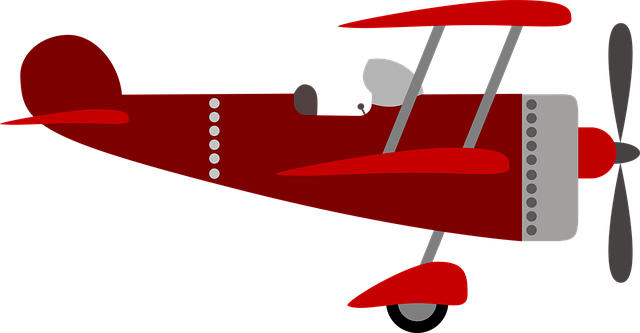
\includegraphics[scale=0.03]{plane}};}

\usepackage{graphicx}

\usepackage{mathtools}

\usepackage{tikz}
\usetikzlibrary{positioning,calc,trees,backgrounds}
\tikzset{%
  inode/.style={%
    thick,
    draw=black,
    ellipse,
    minimum width=30mm,
    minimum height=10mm%
  },
  icnode/.style={%
    thick,
    draw=black,
    circle,
    node distance=5mm
  },
  onode/.style={%
    inode,
    fill=black!40
  },
  ocnode/.style={%
    icnode,
    fill=black!40
  }
}

% A set of styles for overlaying in tikz figures.
% Usage example: style on=<{4,8}>{dashed}
\tikzset{%
  invisible/.style={opacity=0},
  visible on/.style={alt={#1{}{invisible}}},
  style on/.style 2 args={alt={#1#2{}}},
  alt/.code args={<#1>#2#3}{%
    \alt<#1>{\pgfkeysalso{#2}}{\pgfkeysalso{#3}}
  },
}

\title{A Sequential Monte Carlo Example}
\author{Daniel Lundén}

\begin{document}

\frame[plain,t,noframenumbering]{\titlepage}

\begin{frame}{A Model for Aircraft Localization}
  \begin{center}
    \begin{tikzpicture}[trim axis left, trim axis right]
      \begin{axis}[
        width=\textwidth,
        height=6cm,
        aircraft
        ]
        \addplot [mark=plane] file {python/pos_1.dat};
        \only<2->{\addplot [no markers] file {python/map.dat};}
        \only<3->{\addplot [dashed] file {python/dist_1.dat};}
        \end{axis}
      \end{tikzpicture}
    \end{center}
\end{frame}

\begin{frame}{A Model for Aircraft Localization}
  \begin{itemize}
    \item Initial position:
      $X_0 \sim \mathcal{U}(0, 100)$
      \pause
    \item Transition model:
      $X_t \sim \mathcal{N}(X_{t-1} + 2, 0.5)$
      \pause
    \item Observation model:
      $Y_t \sim \mathcal{N}(\text{map}(X_t), 5)$
      \pause
    \item Problem: Find $p(x_t\mid y_{0:t})$
  \end{itemize}
  \pause
  \begin{center}
    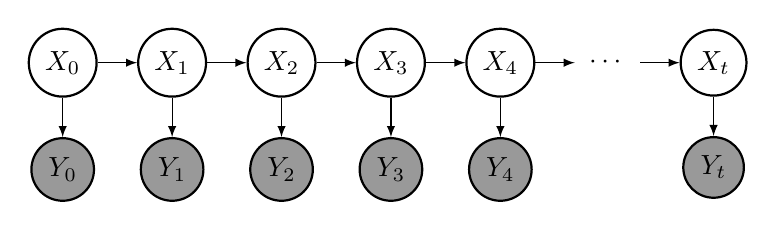
\begin{tikzpicture}
      \node[icnode]                (x0) {$X_0$};
      \node[ocnode, below = of x0] (y0) {$Y_0$};
      \node[icnode, right = of x0] (x1) {$X_1$};
      \node[ocnode, below = of x1] (y1) {$Y_1$};
      \node[icnode, right = of x1] (x2) {$X_2$};
      \node[ocnode, below = of x2] (y2) {$Y_2$};
      \node[icnode, right = of x2] (x3) {$X_3$};
      \node[ocnode, below = of x3] (y3) {$Y_3$};
      \node[icnode, right = of x3] (x4) {$X_4$};
      \node[ocnode, below = of x4] (y4) {$Y_4$};

      \node[icnode, right = of x4, draw=white] (dots) {$\cdots$};

      \node[icnode, right = of dots] (xt) {$X_t$};
      \node[ocnode, below = of xt] (yt) {$Y_t$};
      \path[-latex]
        (x0) edge (x1)
        (x1) edge (x2)
        (x2) edge (x3)
        (x3) edge (x4)
        (x4) edge (dots)
        (dots) edge (xt)
        (x0) edge (y0)
        (x1) edge (y1)
        (x2) edge (y2)
        (x3) edge (y3)
        (x4) edge (y4)
        (xt) edge (yt);
    \end{tikzpicture}
  \end{center}
\end{frame}

\begin{frame}{Importance sampling}
  \begin{center}
    \begin{overprint}
      \only<1>{Initialize 200 samples from $X_0$}
      \only<2,4,6>{Weigh samples using observation model}
      \only<3,5>{Propagate samples using transition model}
      \only<7->{Propagate, weigh}
    \end{overprint}
  \end{center}

  \begin{center}
    \begin{tikzpicture}[trim axis left, trim axis right]
      \begin{axis}[
        width=\textwidth,
        height=6cm,
        aircraft
        ]
        \addplot [no markers] file {python/map.dat};
        \foreach \i in {1,...,3} {%
          \only<+-+(1)>{%
            \addplot [mark=plane] file {python/pos_\i.dat};
            \addplot [dashed] file {python/dist_\i.dat};
            \addplot [dotted] file {python/level_\i.dat};
          }
          \only<+(-1)>{%
            \addplot [particles] file {python/SIS_trans_\i.dat};
          }
          \only<.>{%
            \addplot [particles] file {python/SIS_\i.dat};
          }
        }
        \foreach \i in {4,...,30} {%
          \only<+>{%
            \addplot [mark=plane] file {python/pos_\i.dat};
            \addplot [dashed] file {python/dist_\i.dat};
            \addplot [dotted] file {python/level_\i.dat};
            \addplot [particles] file {python/SIS_\i.dat};
          }
        }
      \end{axis}
    \end{tikzpicture}
  \end{center}
\end{frame}

% Airplane example: introduces Bayesian networks and SMC
\begin{frame}{Sequential Monte Carlo inference}
  \begin{center}
    \begin{overprint}
      \only<1>{Initialize 200 samples from $X_0$}
      \only<2,5,8>{Weigh samples using observation model}
      \only<3,6,9>{Resample}
      \only<4,7>{Propagate samples using transition model}
      \only<10->{Propagate, weigh, resample}
    \end{overprint}
  \end{center}

  \begin{center}
    \begin{tikzpicture}[trim axis left, trim axis right]
      \begin{axis}[
        width=\textwidth,
        height=6cm,
        aircraft
        ]
        \addplot [no markers] file {python/map.dat};
        \foreach \i in {1,...,3} {%
          \only<+-+(2)>{%
            \addplot [mark=plane] file {python/pos_\i.dat};
            \addplot [dashed] file {python/dist_\i.dat};
            \addplot [dotted] file {python/level_\i.dat};
          }
          \only<+(-1)>{%
            \addplot [particles]
              file {python/BPF_trans_\i.dat};
          }
          \only<+(-1)>{%
            \addplot [particles]
              file {python/BPF_\i.dat};
          }
          \only<.>{%
            \addplot [particles]
              file {python/BPF_resample_\i.dat};
          }
        }
        \foreach \i in {4,...,30} {%
          \only<+>{%
            \addplot [mark=plane] file {python/pos_\i.dat};
            \addplot [dashed] file {python/dist_\i.dat};
            \addplot [dotted] file {python/level_\i.dat};
            \addplot [particles] file {python/BPF_resample_\i.dat};
          }
        }
      \end{axis}
    \end{tikzpicture}
  \end{center}
\end{frame}

\end{document}

